\documentclass[border=10pt]{standalone}
\usepackage{tikz}
\usetikzlibrary{shapes.geometric,positioning,arrows.meta,calc}
\begin{document}
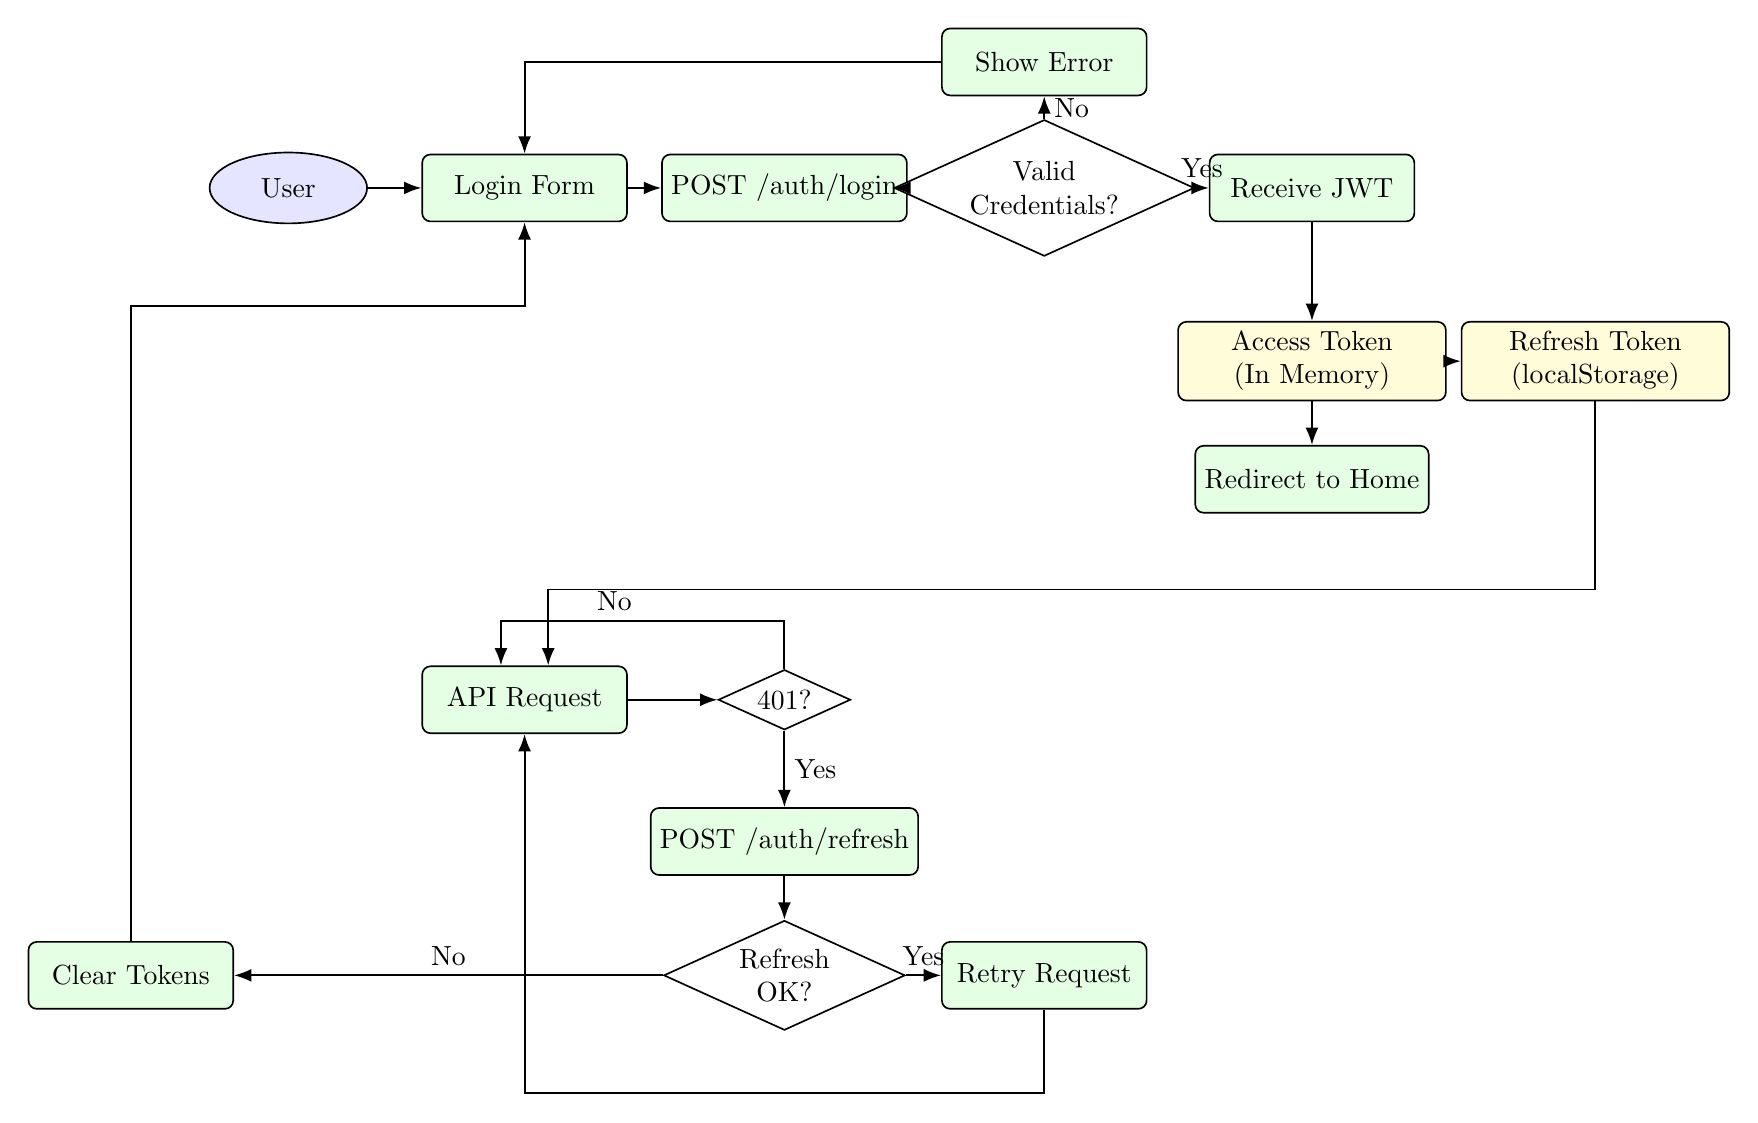
\begin{tikzpicture}[
  font=\normalsize,
  >={Latex[length=2.2mm]},
  process/.style={rounded corners=3pt, draw=black, line width=0.6pt, fill=green!10, minimum width=2.6cm, minimum height=0.85cm, align=center},
  startstop/.style={ellipse, draw=black, line width=0.6pt, fill=blue!10, minimum width=2cm, minimum height=0.9cm, align=center},
  decision/.style={diamond, draw=black, line width=0.6pt, fill=white, aspect=2.2, align=center, inner sep=2pt},
  storage/.style={rounded corners=3pt, draw=black, line width=0.6pt, fill=yellow!15, align=center, minimum width=3.4cm, minimum height=1cm},
  arr/.style={->, line width=0.7pt}
]

%% ============ Row A: Login flow (y = 10) ============
\node[startstop] (user)       at (0,10)    {User};
\node[process]   (loginform)  at (3,10)    {Login Form};
\node[process]   (postlogin)  at (6.3,10)  {POST /auth/login};
\node[decision]  (validcred)  at (9.6,10)  {Valid\\Credentials?};
\node[process]   (showerror)  at (9.6,11.6){Show Error};
\node[process]   (receivejwt) at (13,10)   {Receive JWT};

\draw[arr] (user) -- (loginform);
\draw[arr] (loginform) -- (postlogin);
\draw[arr] (postlogin) -- (validcred);
\draw[arr] (validcred) -- node[right]{No} (showerror);
\draw[arr] (showerror.west) -| (loginform.north);
\draw[arr] (validcred) -- node[above]{Yes} (receivejwt);

%% ============ Rows B/C: Token storage (y = 7.8 / 6.3) ============
\node[storage] (access)   at (13,7.8)   {Access Token\\(In Memory)};
\node[storage] (refresh)  at (16.6,7.8) {Refresh Token\\(localStorage)};
\node[process] (redirect) at (13,6.3)   {Redirect to Home};

\draw[arr] (receivejwt) -- (access);
\draw[arr] (access) -- (refresh);
\draw[arr] (access) -- (redirect);

%% ============ Row D: API request flow (y = 3.5) ============
\node[process]  (apireq) at (3,3.5)   {API Request};
\node[decision] (is401)  at (6.3,3.5) {401?};

%% Refresh token feeds the API request layer; routed through a clear band
%% well below "Redirect to Home" and well above "401?" so it touches no node.
\draw[arr] (refresh.south) -- (16.6,4.9) -| ($(apireq.north)+(0.3,0)$);

\draw[arr] (apireq) -- (is401);

%% ============ Row E/F: Refresh flow (y = 1.7 / 0) ============
\node[process]  (postrefresh) at (6.3,1.7) {POST /auth/refresh};
\node[decision] (refreshok)   at (6.3,0)   {Refresh\\OK?};
\node[process]  (retry)       at (9.6,0)   {Retry Request};
\node[process]  (clear)       at (-2,0)    {Clear Tokens};

\draw[arr] (is401) -- node[right]{Yes} (postrefresh);
\draw[arr] (postrefresh) -- (refreshok);
\draw[arr] (refreshok) -- node[above]{Yes} (retry);
\draw[arr] (refreshok) -- node[above]{No} (clear);

%% 401? "No" loop: small arc above 401?, clear of the refresh-feed band above it
\draw[arr] (is401.north) -- (6.3,4.5) -| node[pos=0.3, above]{No} ($(apireq.north)+(-0.3,0)$);

%% Retry Request loop: dips below the row, runs left, rejoins API Request from below
\draw[arr] (retry.south) -- (9.6,-1.5) -| (apireq.south);

%% Clear Tokens -> back to Login Form: runs up the far-left margin, jogs in
%% above everything else so it never crosses API Request's column
\draw[arr] (clear.north) -- (-2,8.5) -| (loginform.south);

\end{tikzpicture}
\end{document}
